% Figure 2: OTLP Type System Overview
% Author: OTLP Project
% Date: October 20, 2025

\begin{figure}[t]
\centering
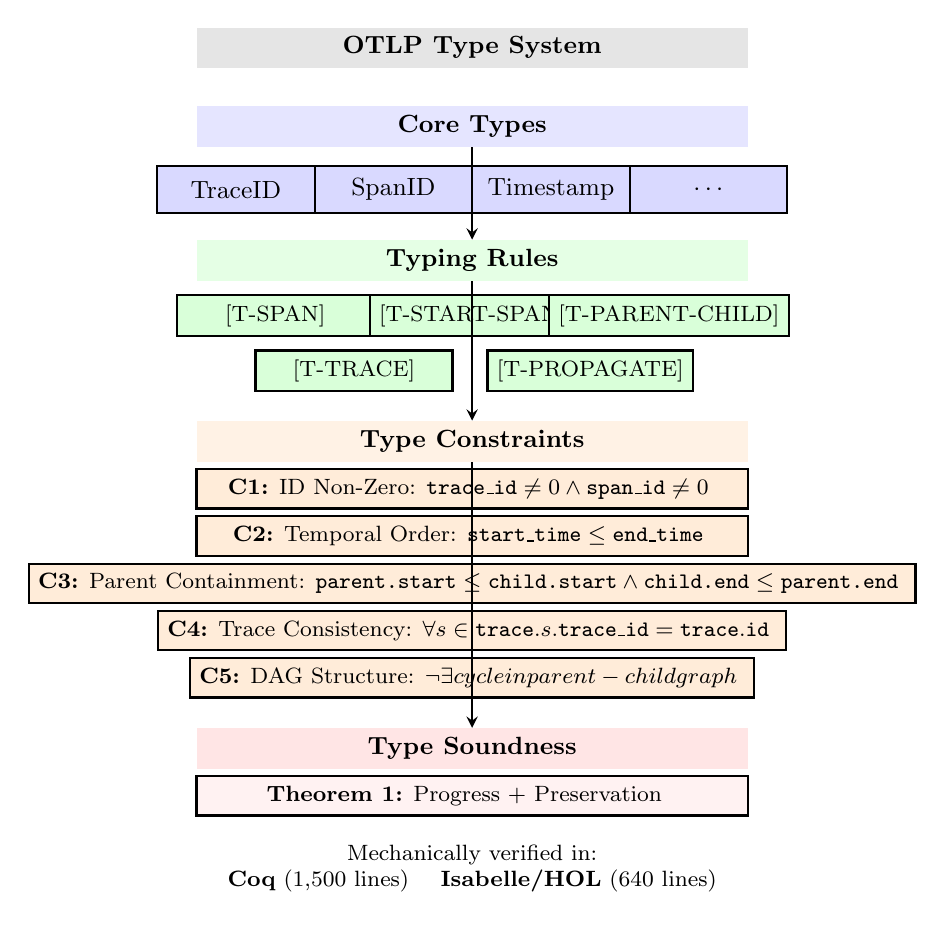
\begin{tikzpicture}[
    node distance=0.8cm,
    typebox/.style={rectangle, draw, thick, fill=blue!15, minimum width=2cm, minimum height=0.6cm, align=center, font=\small},
    rulebox/.style={rectangle, draw, thick, fill=green!15, minimum width=2.5cm, minimum height=0.5cm, align=center, font=\footnotesize},
    constraintbox/.style={rectangle, draw, thick, fill=orange!15, minimum width=7cm, minimum height=0.5cm, align=left, font=\footnotesize},
    titlebox/.style={rectangle, fill=gray!20, minimum width=7cm, minimum height=0.4cm, align=center, font=\small\bfseries}
]

% Title
\node[titlebox] (title) at (0, 5.5) {OTLP Type System};

% Core Types Section
\node[titlebox, fill=blue!10] (coretitle) at (0, 4.5) {Core Types};

\node[typebox] (traceid) at (-3, 3.7) {TraceID};
\node[typebox] (spanid) at (-1, 3.7) {SpanID};
\node[typebox] (timestamp) at (1, 3.7) {Timestamp};
\node[typebox] (etc) at (3, 3.7) {$\cdots$};

% Typing Rules Section
\node[titlebox, fill=green!10] (ruletitle) at (0, 2.8) {Typing Rules};

\node[rulebox] (tspan) at (-2.5, 2.1) {[T-SPAN]};
\node[rulebox] (tstart) at (0, 2.1) {[T-START-SPAN]};
\node[rulebox] (tparent) at (2.5, 2.1) {[T-PARENT-CHILD]};

\node[rulebox] (ttrace) at (-1.5, 1.4) {[T-TRACE]};
\node[rulebox] (tprop) at (1.5, 1.4) {[T-PROPAGATE]};

% Type Constraints Section
\node[titlebox, fill=orange!10] (consttitle) at (0, 0.5) {Type Constraints};

\node[constraintbox] (c1) at (0, -0.1) {
    \textbf{C1:} ID Non-Zero: $\texttt{trace\_id} \neq 0 \land \texttt{span\_id} \neq 0$
};

\node[constraintbox] (c2) at (0, -0.7) {
    \textbf{C2:} Temporal Order: $\texttt{start\_time} \leq \texttt{end\_time}$
};

\node[constraintbox] (c3) at (0, -1.3) {
    \textbf{C3:} Parent Containment: $\texttt{parent.start} \leq \texttt{child.start} \land \texttt{child.end} \leq \texttt{parent.end}$
};

\node[constraintbox] (c4) at (0, -1.9) {
    \textbf{C4:} Trace Consistency: $\forall s \in \texttt{trace}. s.\texttt{trace\_id} = \texttt{trace}.\texttt{id}$
};

\node[constraintbox] (c5) at (0, -2.5) {
    \textbf{C5:} DAG Structure: $\neg\exists\text{ cycle in parent-child graph}$
};

% Soundness Section
\node[titlebox, fill=red!10] (soundtitle) at (0, -3.4) {Type Soundness};

\node[constraintbox, fill=red!5] (soundness) at (0, -4.0) {
    \textbf{Theorem 1:} Progress + Preservation $\checkmark$
};

\node[below, align=center, font=\footnotesize] at (0, -4.5) {
    Mechanically verified in:\\
    \textbf{Coq} (1,500 lines) \quad \textbf{Isabelle/HOL} (640 lines)
};

% Arrows
\draw[->, >=stealth, thick] (coretitle.south) -- (ruletitle.north);
\draw[->, >=stealth, thick] (ruletitle.south) -- (consttitle.north);
\draw[->, >=stealth, thick] (consttitle.south) -- (soundtitle.north);

% Side annotations with checkmarks
\node[right, font=\tiny, align=left, green!50!black] at (3.7, -0.1) {$\checkmark$};
\node[right, font=\tiny, align=left, green!50!black] at (3.7, -0.7) {$\checkmark$};
\node[right, font=\tiny, align=left, green!50!black] at (3.7, -1.3) {$\checkmark$};
\node[right, font=\tiny, align=left, green!50!black] at (3.7, -1.9) {$\checkmark$};
\node[right, font=\tiny, align=left, green!50!black] at (3.7, -2.5) {$\checkmark$};

\end{tikzpicture}
\caption{OTLP Type System overview showing core types, typing rules, and five critical constraints (C1-C5). The type system enforces protocol correctness through static typing rules that govern span creation, parent-child relationships, and trace assembly. Type soundness is proven through Progress and Preservation theorems (Theorem 1), mechanically verified in Coq (1,500 lines) and Isabelle/HOL (640 lines). All constraints are statically checkable, enabling early error detection before trace export.}
\label{fig:type-system}
\end{figure}

